\chapter{Diseño del sistema}
\label{chap:disenosistema}
En este capítulo se describirá el diseño del sistema desarrollado. 
En la sección 3.1 se detallará la arquitectura del sistema global. 
En el apartado 3.2 se profundizará en la arquitectura interna del HUB.
\lsection{Necesidades del sistema}
En esta sección se analizarán las necesidades de nuestro sistema y los dispositivos con los que nos comunicaremos.
\subsection{Necesidades de los dispositivos}
Antes de empezar a diseñar el sistema y elegir el protocolo que se utilizará y el medio físico por el que se comunicarán 
nuestros dispositivos es necesario analizar los dispositivos que podrán conectarse a nuestro HUB así como sus necesidades. 
Una vez determinados los requisitos del protocolo se estudiará el medio físico de comunicación.
\newline
\newline
Los principales dispositivos domóticos que hemos encontrado son: sensores de temperatura, sensores de humedad, 
sensores de luz, sensores de movimiento, medidores de distancia, sensores de humo, sensores magnéticos, cámaras, 
bombillas, enchufes, termostatos, motores, aires acondicionados, interruptores y altavoces.
\newline
Estos dispositivos pueden ser divididos en dos grupos: sensores y actuadores. 
\newline
Los sensores solamente envían determinada información a nuestro HUB (comunicación unidireccional), 
mientras que los actuadores reciben mensajes con determinados comandos a parte de enviar información del estado 
en el que se encuentran (comunicación bidireccional).

Agrupación de los dispositivos encontrados:

\begin{figure}[H]
\centering
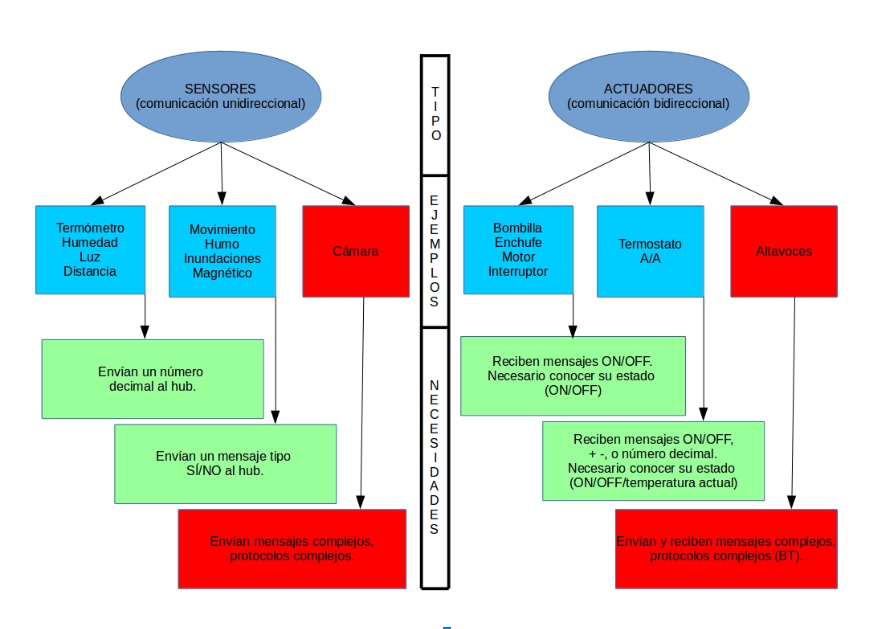
\includegraphics[width=6.00in]{images/descripcion_dispositivos.png}
\caption{Tipos de dispositivos}
\label{fig:descripcion_dispositivos}
\end{figure}


Para la definición del protocolo dividiremos los dispositivos en tres tipos:
\begin{itemize}
\item Tipo 1 (sensores): el hub sólo recibe información de los sensores. El hub no necesita saber qué tipo de información recoge (número decimal, SÍ/NO...etc), simplemente la actualiza y la muestra al usuario.
\item Tipo 2 (actuadores): estos dispositivos envían información al HUB y son capaces de recibir comandos tipo ON/OFF, +/-, número decimal...etc.
\item Tipo 3: cámaras IP. Este sensor recibirá un tratamiento especial debido a la necesidad de una comunicación constante y rápida.
\end{itemize}
\subsection{Necesidades del sistema}
Una vez analizadas las necesidades de los dispositivos podemos analizar las necesidades de nuestro sistema.
Para el desarrollo de nuestro sistema necesitaremos una arquitectura que nos permita:
\begin{itemize}
\item Comunicación bidireccional entre los dispositivos y el hub: es necesario que el hub conozca información de los dispositivos, 
registre dispositivos y gestione dispositivos, así como también es necesario que los dispositivos puedan recibir comandos provenientes
del hub. El hub debe permitir aceptar dispositivos con diferentes comandos, y no ceñirse sólo a un número cerrado de comandos (ON/OFF, +/-,...).
\item Comunicación entre el hub y la interfaz: será necesario que la información de los dispositivos y el estado de los mismos sea accesible
a través de la interfaz de usuario. Además el usuario debe ser capaz de gestionar los dispositivos y enviar comandos a los actuadores
a través de la interfaz.
\item Seguridad en la comunicación: es imprescindible que toda comunicación se realice de manera segura, de tal manera que nadie pueda modificar o
acceder a nuestra información.
\item Escalabilidad: aunque durante la realización de nuestro proyecto nos centraremos únicamente en la comunicación mediante protocolo HTTPS, 
es necesario diseñar un sistema escalable que el día de mañana pueda funcionar con diferentes protocolos y dispositivos.
\end{itemize}
\lsection{Protocolos}
En esta sección se describirá el protocolo que se utilizará en las comunicaciones entre los dispositivos y el HUB.
\subsection{Protocolo HTTPS}
El protocolo elegido para la comunicación entre dispositivos, hub e interfaz es el protocolo HTTPS (Hypertext Transfer Protocol Secure).
\newline
Este protocolo nos da la posibilidad de implementar una API REST consumible por parte de los dispositivos y por parte de la interfaz,
sin necesidad de utilizar diferentes protocolos para los diferentes canales. 
\newline
Además, de estar muy estandarizadas a día de hoy, las APIs REST nos dan la capacidad de separar entre cliente y servidor y de ser capaces
de utilizar diferentes lenguajes y tecnologías para cada lado. Es decir, podemos tener un servidor escrito en Express.js (javascript), una interfaz 
gráfica utilizando Angular5 (TypeScript), y unos actuadores/sensores que utilicen CherryPy (Python).
\newline
Además, utilizar HTTPS nos ofrece la posibilidad de crear un canal de comunicación cifrado, de manera que la información que circula en dicho 
canal no pueda ser descifrada por ningún intermediario ni se pueda sufrir un ataque Man-In-The-Middle*.
\lsection{Arquitectura del sistema}
En esta sección se describirá el diseño y la arquitectura del sistema de manera global, incluyendo dispositivos actuadores, 
dispositivos sensores y el propio hub.
\subsection{Arquitectura del sistema}
Teniendo en cuenta las necesidades de nuestro sistema realizaremos una arquitectura similar a las arquitecturas de microservicios,
en la que el hub y los actuadores serán los hosts de un servidor REST y serán capaces de recibir y procesar peticiones.
\newline
El hub recibirá peticiones de parte de la interfaz y de los dispositivos, y lanzará peticiones a los actuadores. Para ello se establecerá una API consumible por ambas partes (dispositivos e interfaz).
Los sensores lanzarán peticiones al hub informando de su estado.
Los actuadores, además de lanzar peticiones al hub para informar de su estado, deberán ser capaces de recibir peticiones del hub con
diferentes comandos.

Todas las peticiones deben ser securizadas, y debemos asegurar que ningún intruso pueda acceder y/o modificar la información de nuestro sistema.

Esquema de la arquitecura a seguir:
\begin{figure}[H]
\centering
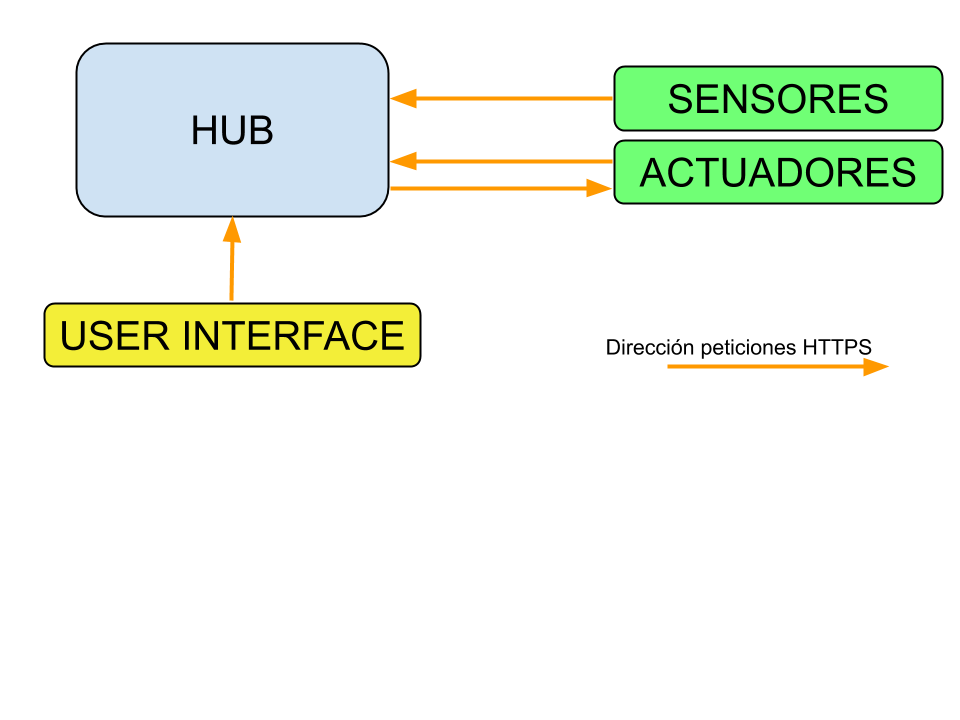
\includegraphics[width=6.00in]{images/esquema_arquitectura.png}
\caption{Tipos de dispositivos}
\label{fig:descripcion_dispositivos}
\end{figure}

\subsection{API}

\lsection{Arquitectura del hub}
\subsection{Módulos}
\subsection{Bases de datos}

